\documentclass{article}
\usepackage{graphicx,float}
\usepackage{amsmath,latexsym,amsfonts,amssymb,amsthm}

\usepackage[utf8]{inputenc}
\usepackage[english]{babel}
\usepackage[letterpaper,top=2cm,bottom=2cm,left=3cm,right=3cm,marginparwidth=1.75cm]{geometry}
\renewcommand{\baselinestretch}{1.667}


\title{Compute Intelligence PS s7 Lab 2}
\author{Joris Plaščinskas}
\date{\today}


\begin{document}


    \maketitle
    \section*{Introduction}
        The goal of this laboratory work is to explore ML classification problems and gradient descent algorithm. My student number is 2016020, which means that I will be using batch gradient descent and a sigmoid function. I will be exploring to datasets: Iris and Breast Cancer Wisconsin. Each data-point in iris database is a plant. Iris dataset is one of the earliest datasets (1936) used in the literature on classification methods and is a popular choice for learning ML. Each data-point is classified into one of three classes which all represent a type of iris plant. Each data-point in Breast Cancer Wisconsin dataset represents a tumor that is either benign (0) or malignant (1)

    \section*{Code}
        The code is split into two parts: refine data and model training and execution.
        \subsection*{Refining Data}
            \textbf{Breast Cancer Wisconsin (in total 683 data-points with 9  features)}
            Using code I removed unnecessary columns and rows that contained missing values and relabeled the tumor class. \\
            \textbf{Iris (in total 500 data-points with 4 features)}
            One of the requirements was to create artificial data-points for Iris dataset. I did this by generating a random value for each feature between it's min and max. Also since we are doing a binary classification model, I only left the 'versicolor' and 'virginica' species. The images below show how the original Iris and artificial Iris datasets are distributed.
            \begin{figure}[H]
                \centering
                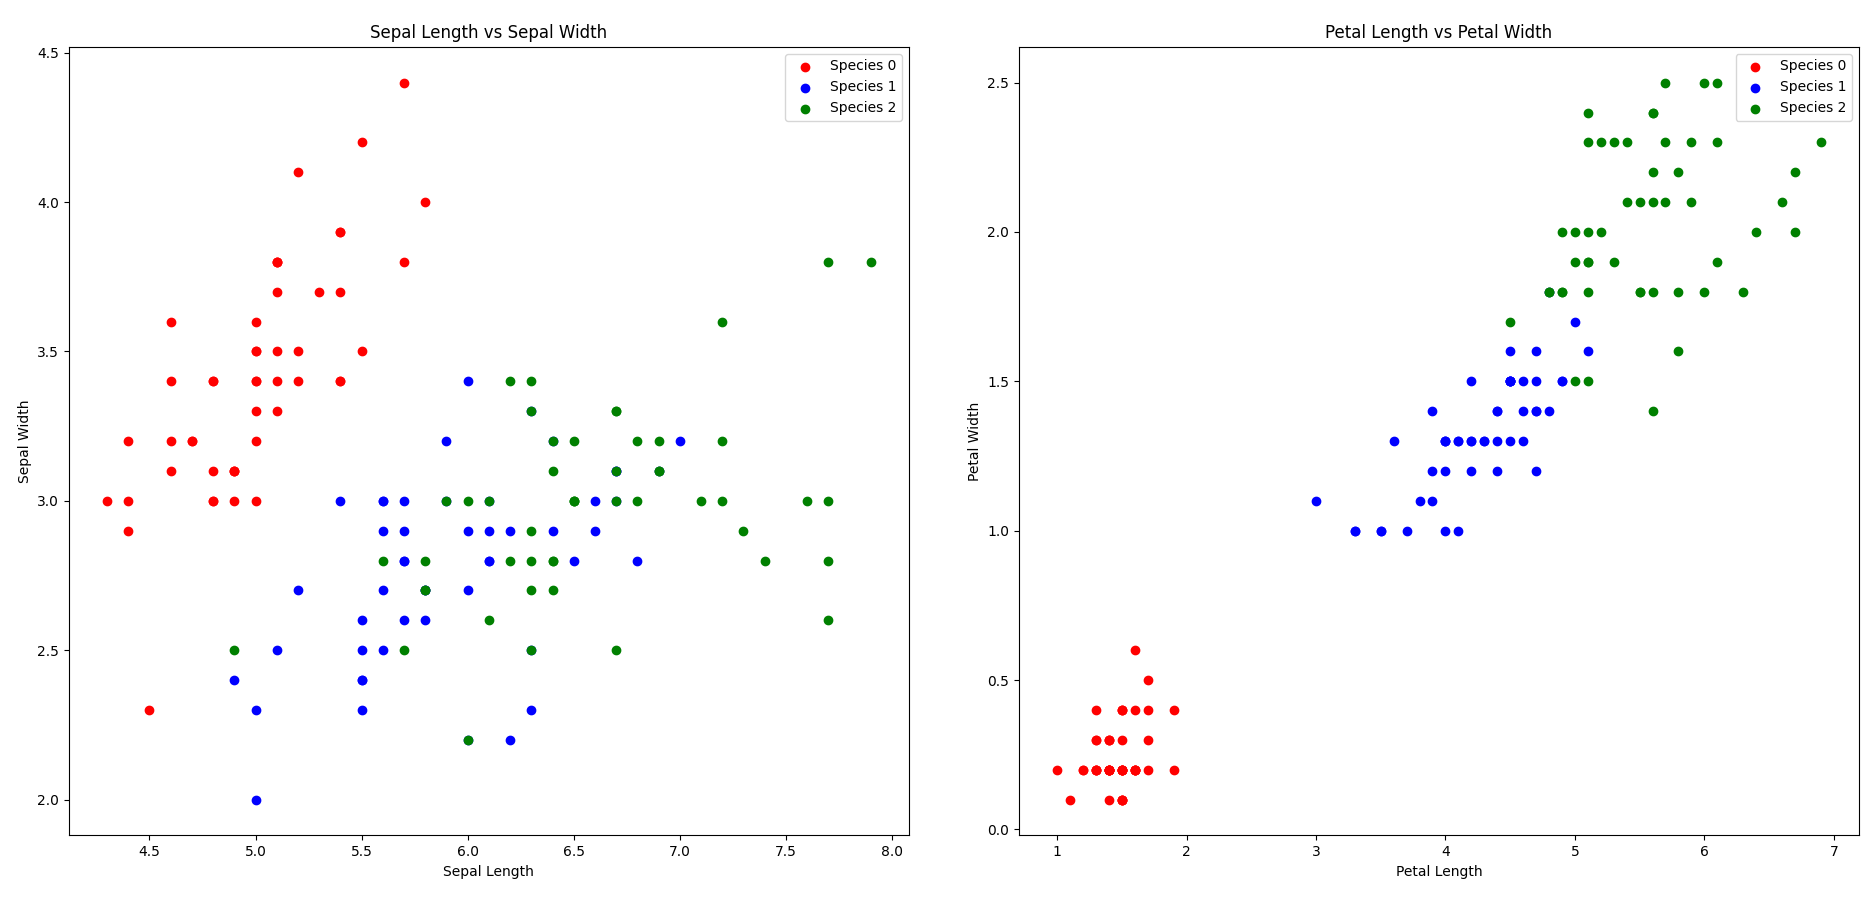
\includegraphics[width=0.7\textwidth]{iris.png}
                \caption{Iris Original Data Distribution}
            \end{figure}
            \begin{figure}[H]
                \centering
                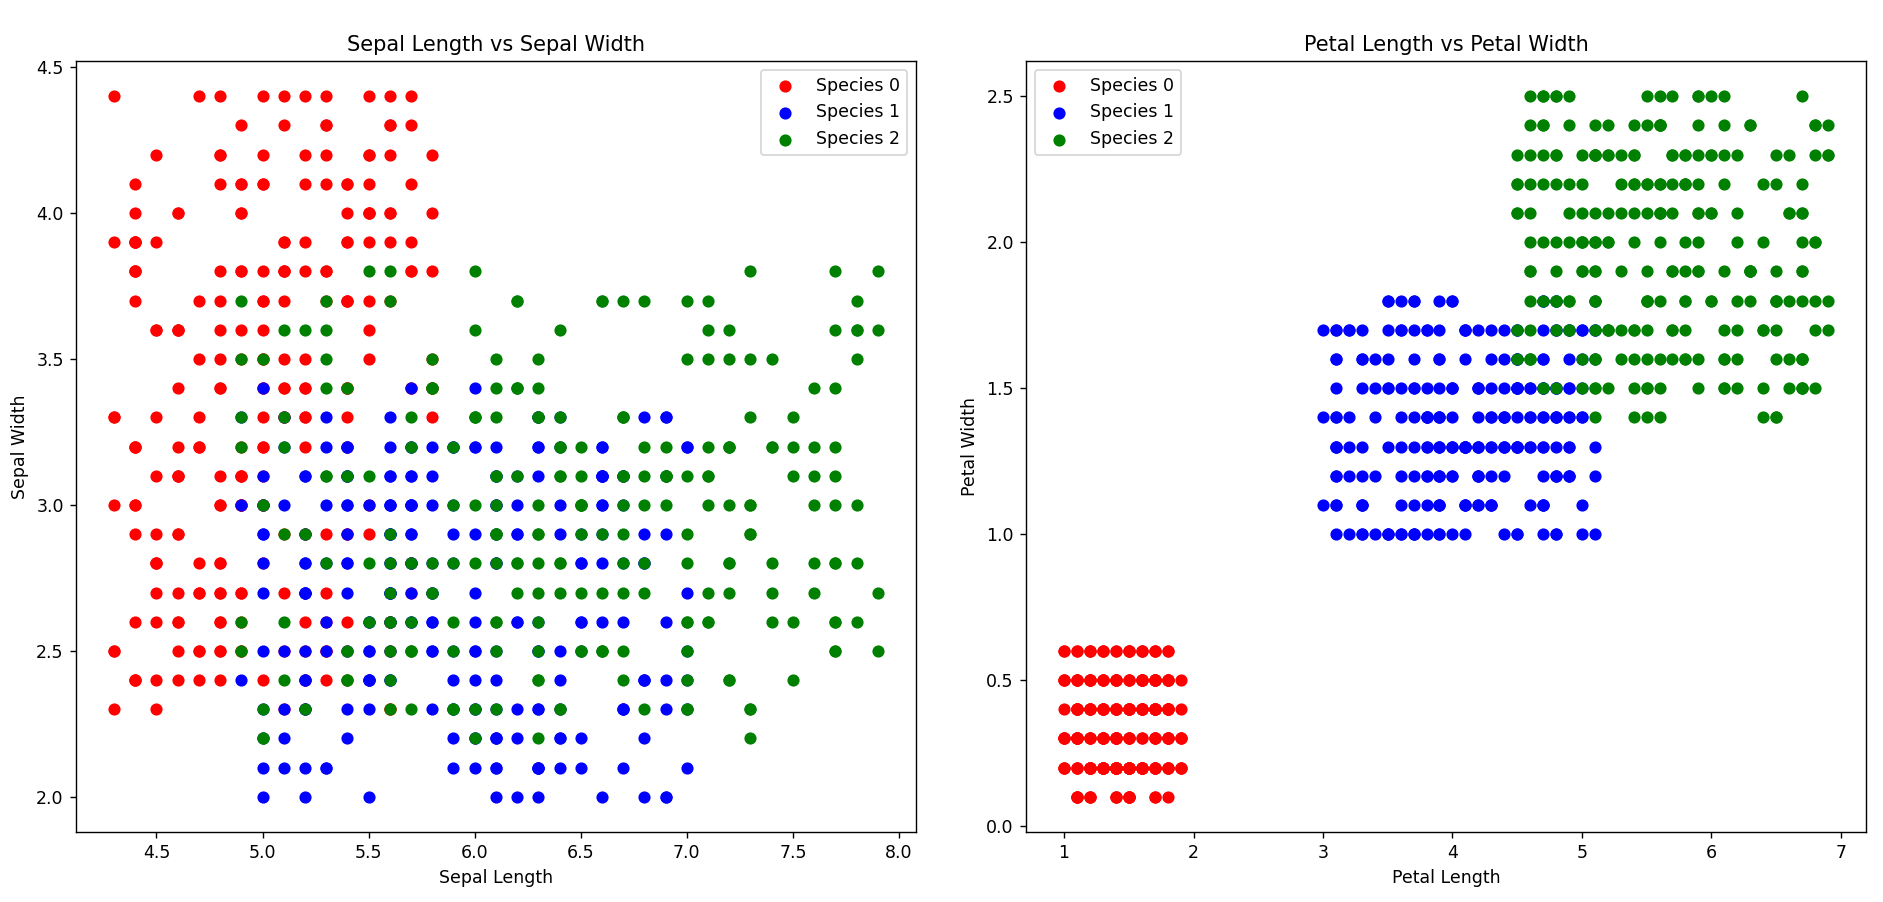
\includegraphics[width=0.7\textwidth]{iris-combined.png}
                \caption{Iris Artificial Data Distribution}
            \end{figure}
        \subsection*{Model Training and Execution}
            For this laboratory work I decided to only use 'numpy' and 'autograd' libraries, so that I could better understand the optimization methods used behind ML. I also chose not to use a sigmoid function on top of my neuron output, because that lead to very poor results.
            \begin{figure}[H]
                \centering
                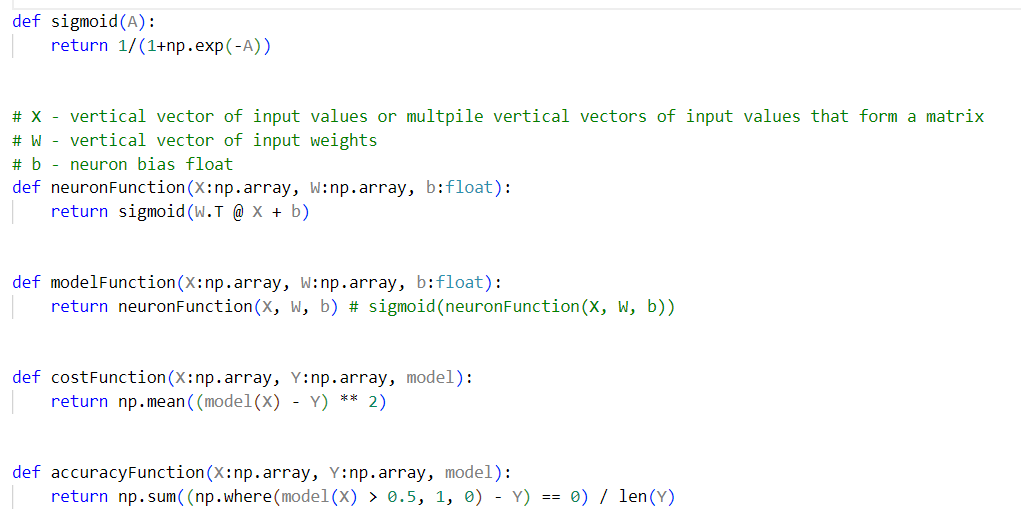
\includegraphics[width=1\textwidth]{functions.png}
                \caption{ML Functions}
                \label{fig:functions}
            \end{figure}
            The first 80\% of the data was put into the training set and the rest into the test set. I then created the accuracy and cost measuring functions for both sets and found the training set cost function derivative using 'autograd'. I initialized $\vec{w}$ and $b$ parameters to random values.
            \begin{figure}[H]
                \centering
                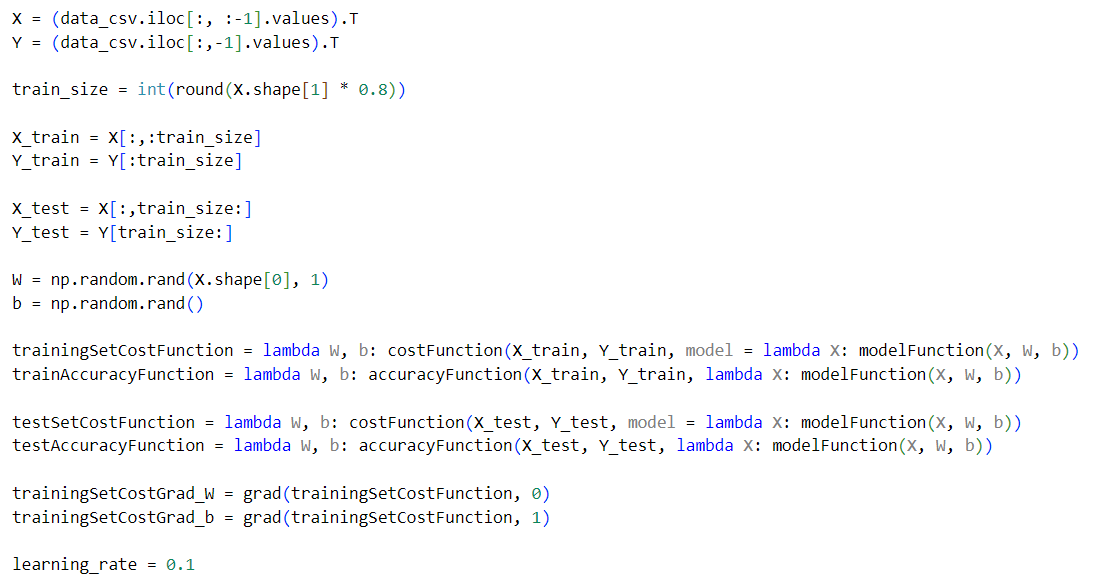
\includegraphics[width=1\textwidth]{data-split.png}
                \caption{Data and Functions Preparation}
                \label{fig:data-split}
            \end{figure}
            Finally I wrote the gradient descent training loop, which involves calculating two gradients, because I had parameters $\vec{w}$ and $b$ separated.
            \begin{figure}[H]
                \centering
                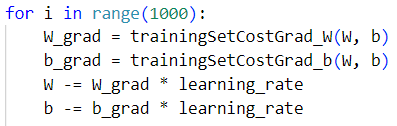
\includegraphics[width=0.7\textwidth]{training-loop.png}
                \caption{Training Loop}
                \label{fig:training-loop}
            \end{figure}

    \section*{Results}
        \subsection*{Breast Cancer Wisconsin}
            The 4 graphs below show the accuracy and cost over each training epoch. These results were obtained with learning rate equals to 1 and 100 epochs. It's very visible from the bumps in the graphs that with such a high learning rate the descent isn't stable (but it works). Looking at figures \ref{fig:cancer-train-cost} and \ref{fig:cancer-train-acc} we can see that the accuracy graph results are very much related to the cost graph - the lower the cost is the better the model performs. Test and training cost graphs are almost identical (\ref{fig:cancer-train-cost} and \ref{fig:cancer-test-cost}), which means that the model should perform well on new data as well.
            \begin{figure}[H]
                \centering
                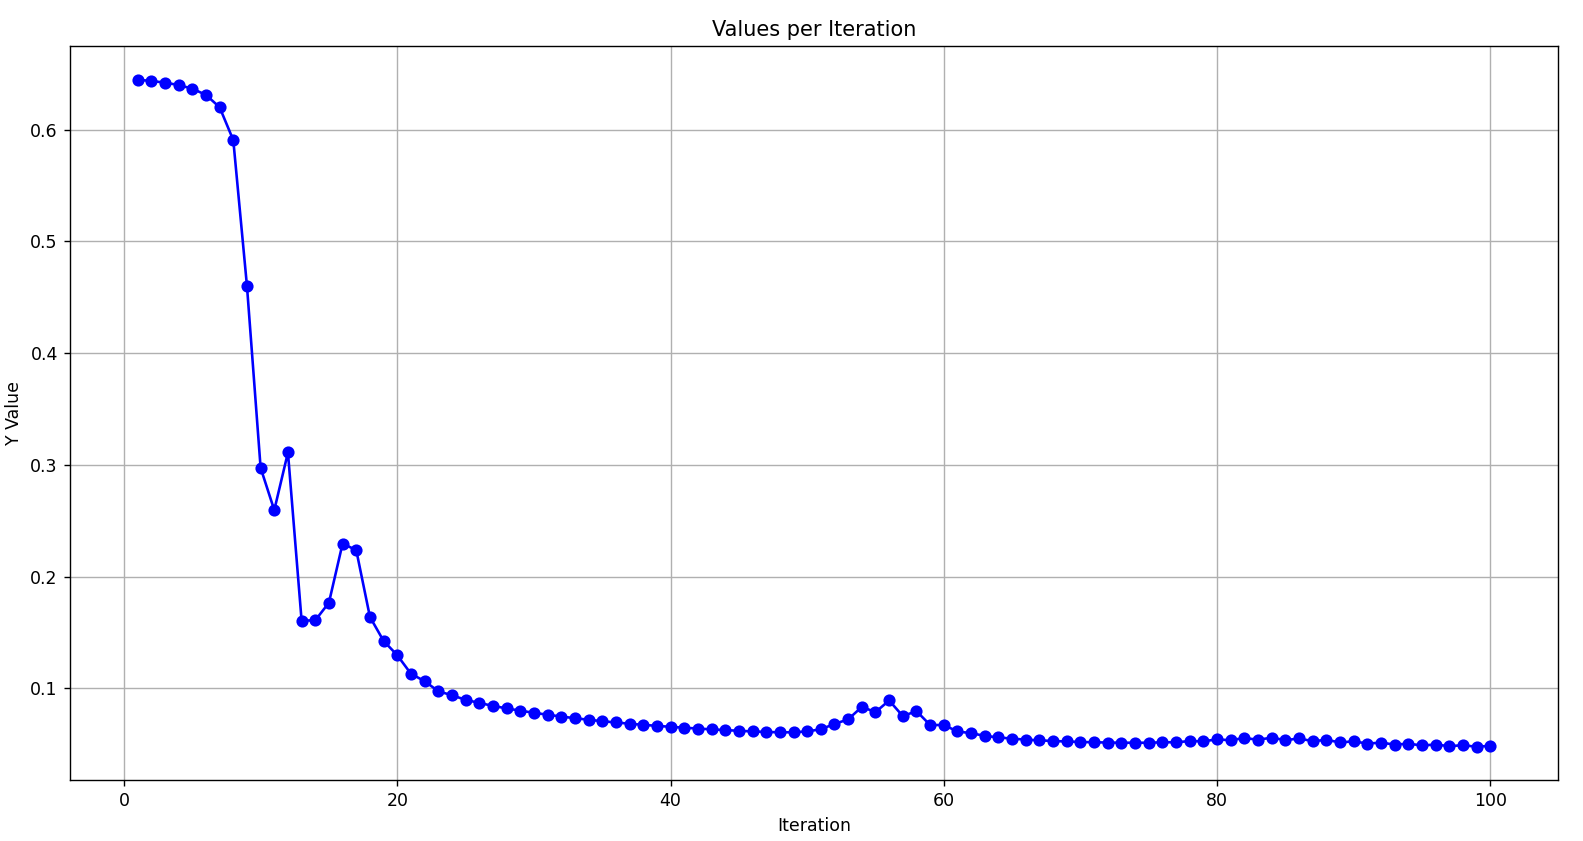
\includegraphics[width=0.7\textwidth]{cancer-train-cost.png}
                \caption{Training Cost}
                \label{fig:cancer-train-cost}
            \end{figure}
            \begin{figure}[H]
                \centering
                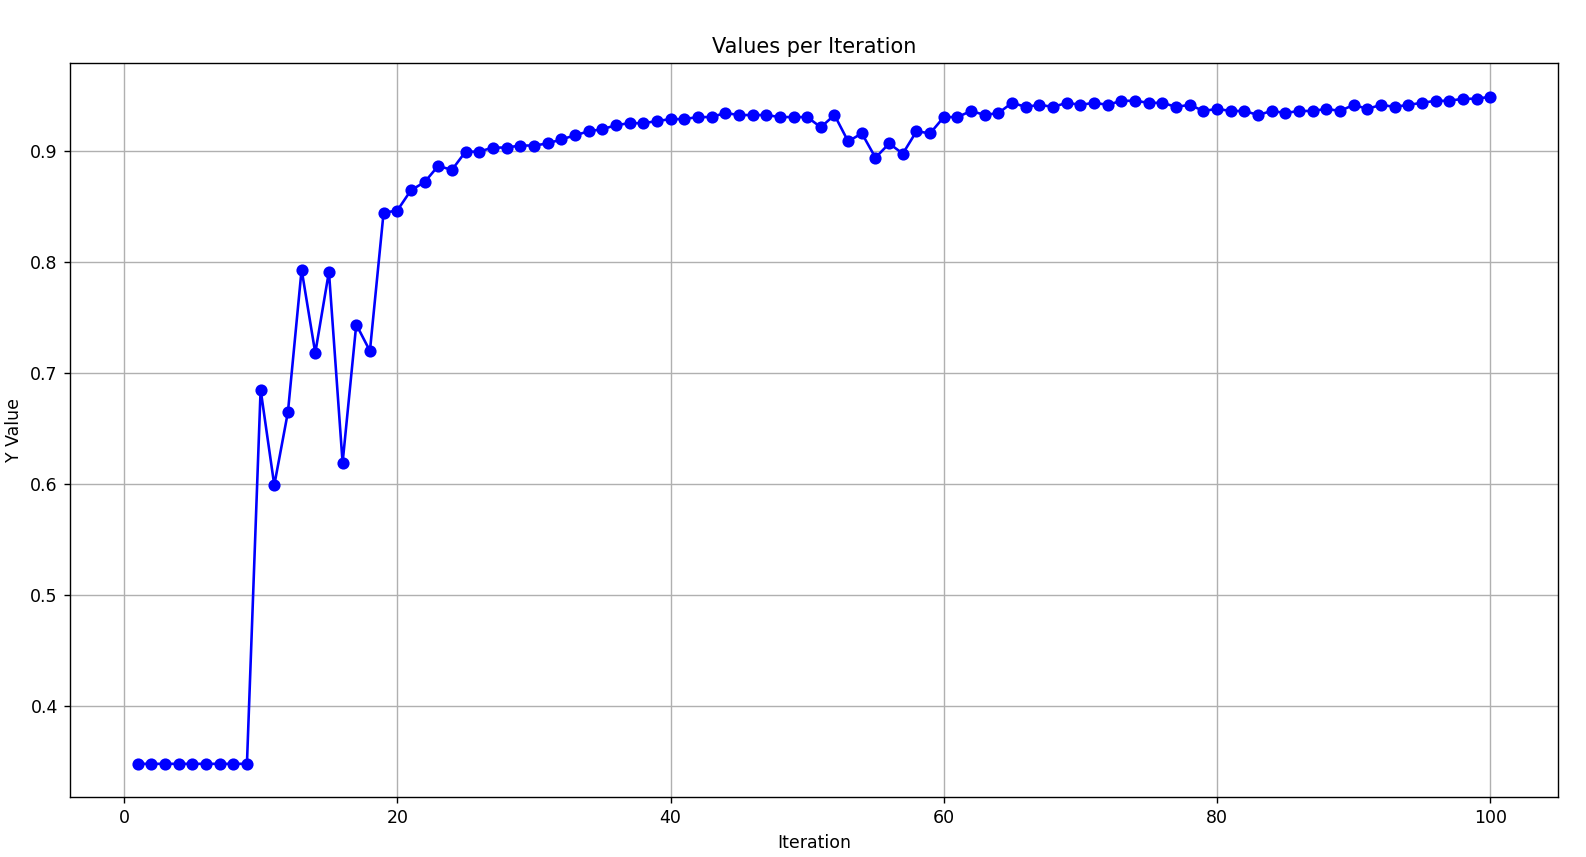
\includegraphics[width=0.7\textwidth]{cancer-train-acc.png}
                \caption{Training Accuracy}
                \label{fig:cancer-train-acc}
            \end{figure}
            \begin{figure}[H]
                \centering
                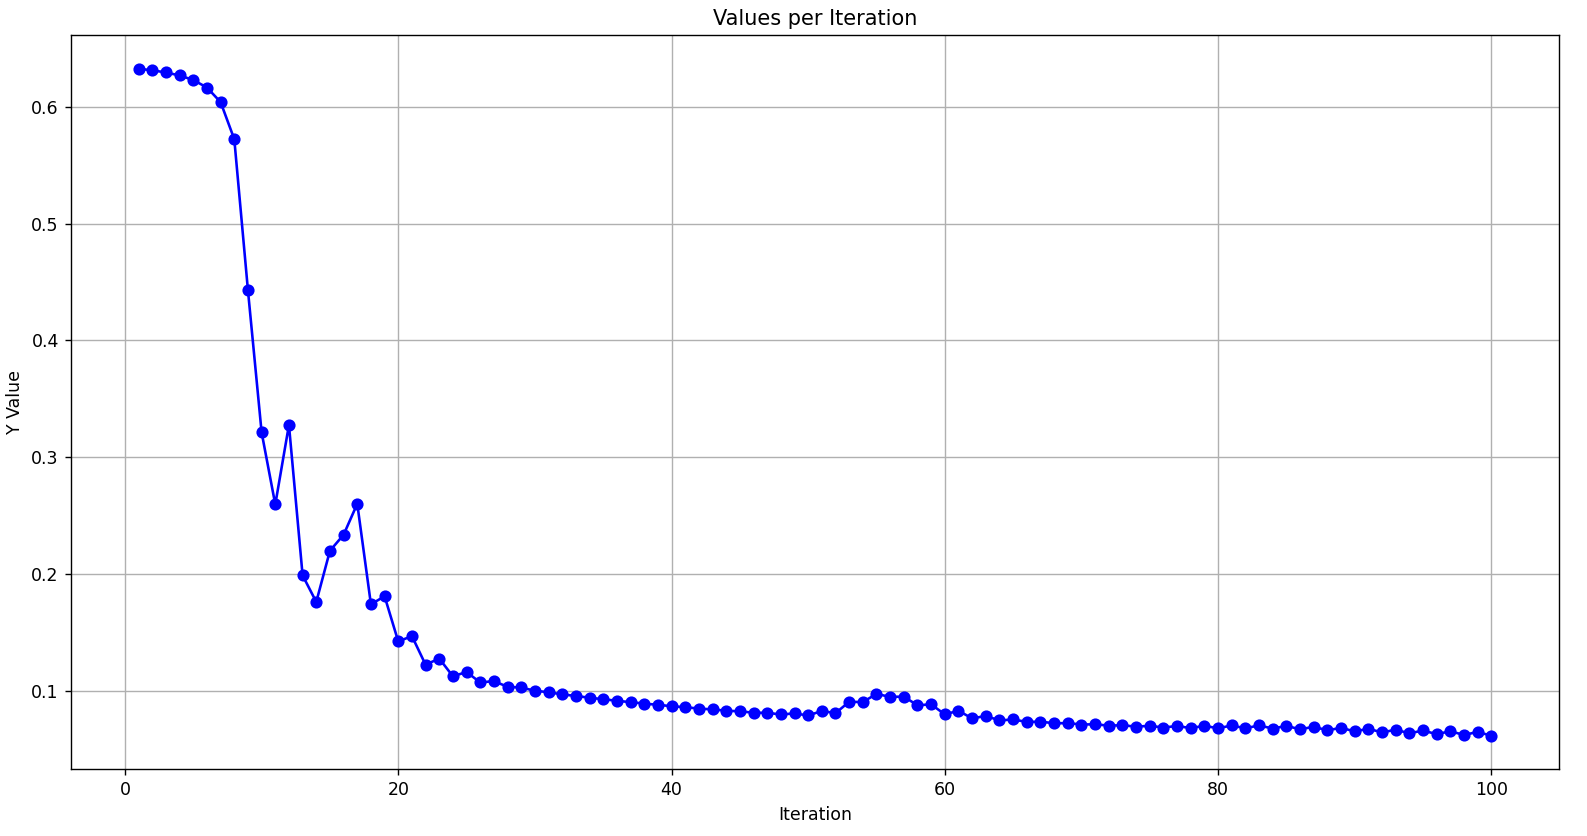
\includegraphics[width=0.7\textwidth]{cancer-test-cost.png}
                \caption{Test Cost}
                \label{fig:cancer-test-cost}
            \end{figure}
            \begin{figure}[H]
                \centering
                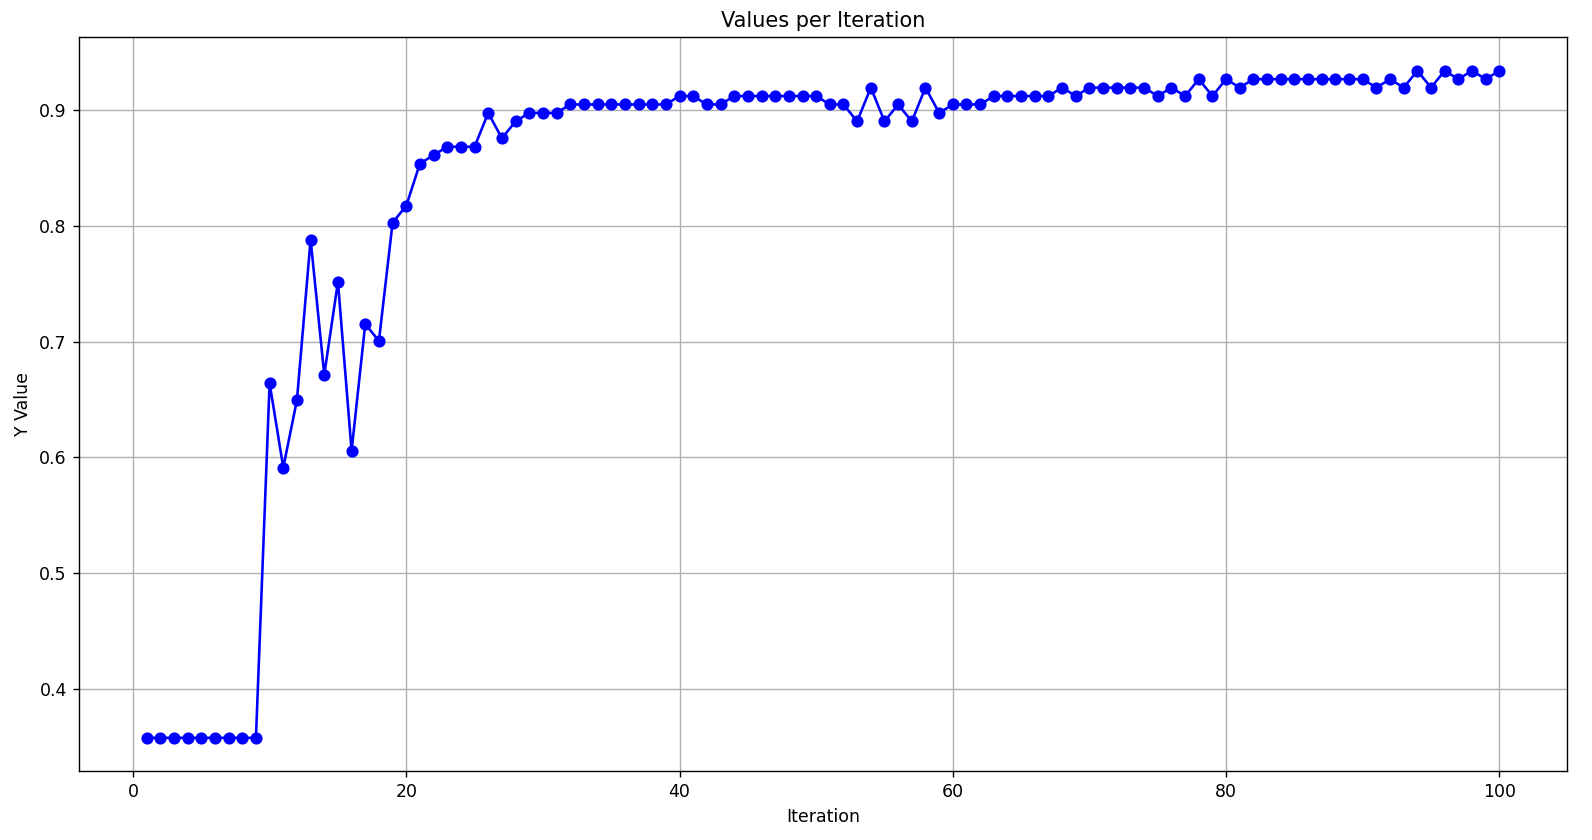
\includegraphics[width=0.7\textwidth]{cancer-test-acc.png}
                \caption{Test Accuracy}
                \label{fig:cancer-test-acc}
            \end{figure}
            The graph below shows the training cost using a $0.1$ learning rate and $1000$ epochs. We can see that the descent is a lot smoother.
            \begin{figure}[H]
                \centering
                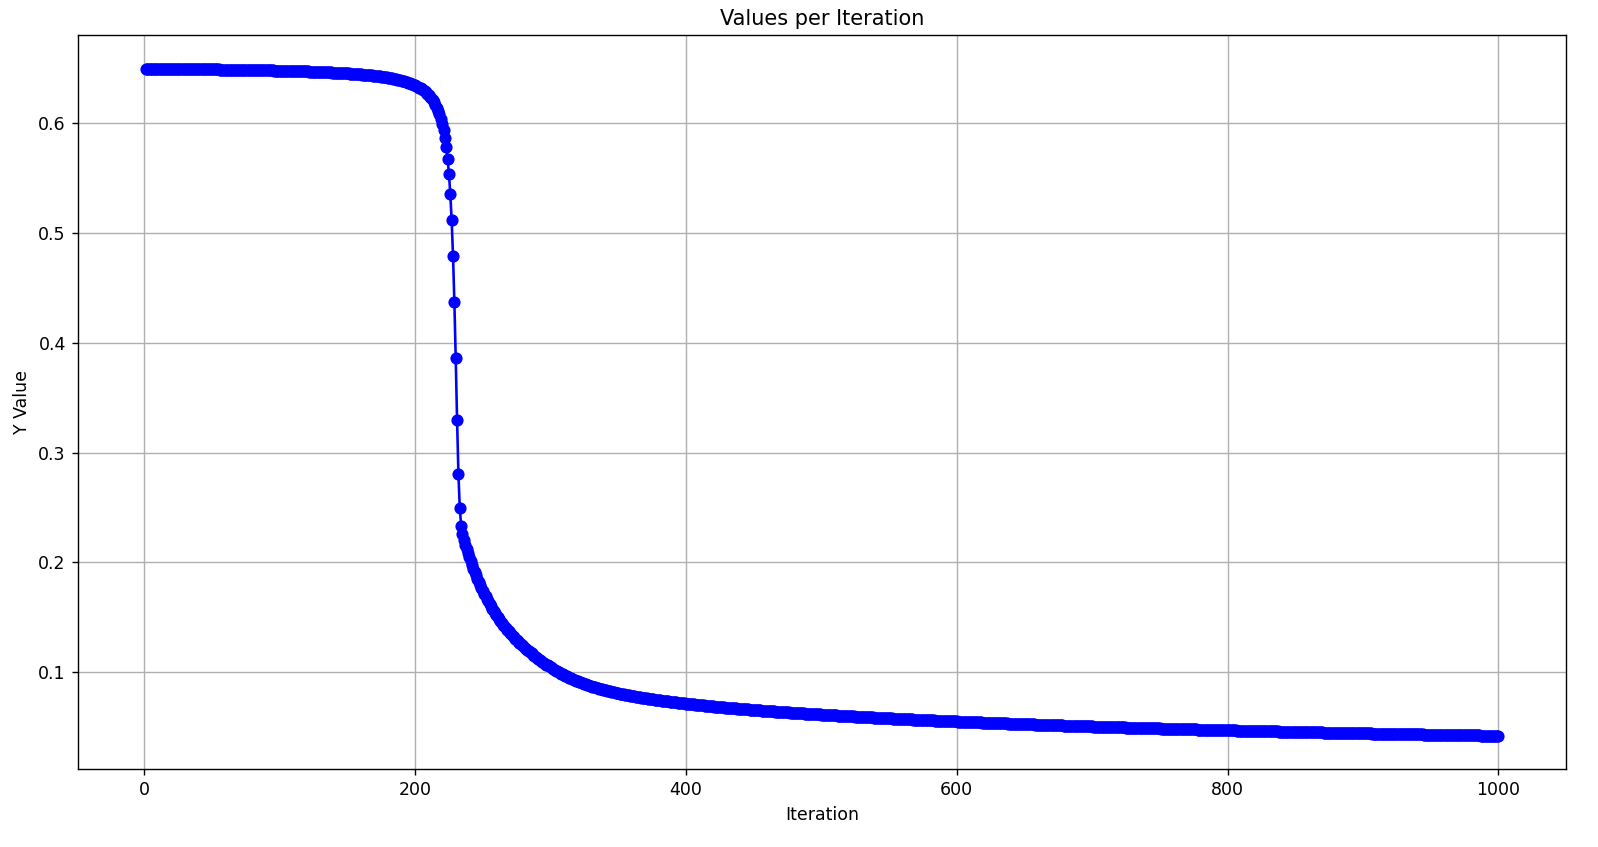
\includegraphics[width=0.7\textwidth]{cancer-low-lr.png}
                \caption{Low Learning Rate, Many Epochs Training Cost}
            \end{figure}
            Finally, the results highly depend on the initial values of $\vec{w}$ and $b$, during some runs the cost function just got stuck at a local minimum or a saddle point as seen in figure-\ref{fig:cancer-sadle}.
            \begin{figure}[H]
                \centering
                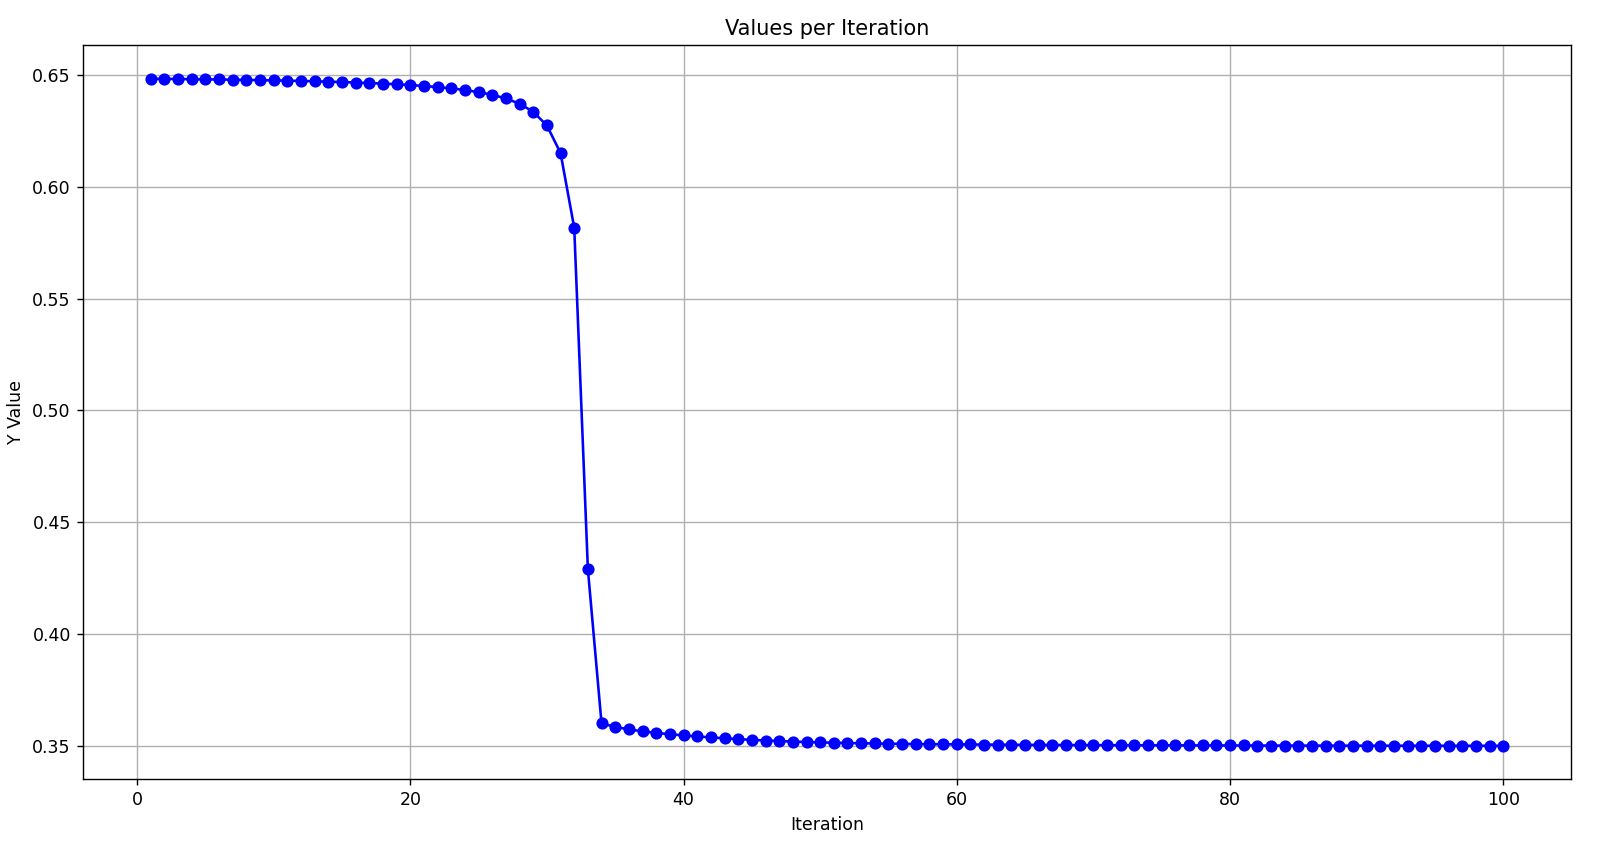
\includegraphics[width=0.7\textwidth]{cancer-sadle.png}
                \caption{Failed Run}
                \label{fig:cancer-sadle}
            \end{figure}
            The weights and bias obtained after training with a learning rate of 1 and 100 epochs are seen in figure-\ref{fig:cancer-results}.
            \begin{figure}[H]
                \centering
                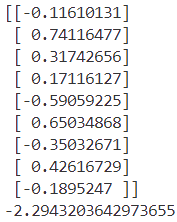
\includegraphics[width=0.4\textwidth]{cancer-results.png}
                \caption{$\vec{w}$ and b values}
                \label{fig:cancer-results}
            \end{figure}
        \subsection*{Iris}
            Training on Iris dataset required using a smaller learning rate than 1, because the descent was very unstable when using 1, so I ended up using $10000$ epochs and a $0.001$ learning rate for the Iris dataset. The 4 graphs below are very similar in shape to the Breast Cancer graphs, so the same insights apply here. 
            \begin{figure}[H]
                \centering
                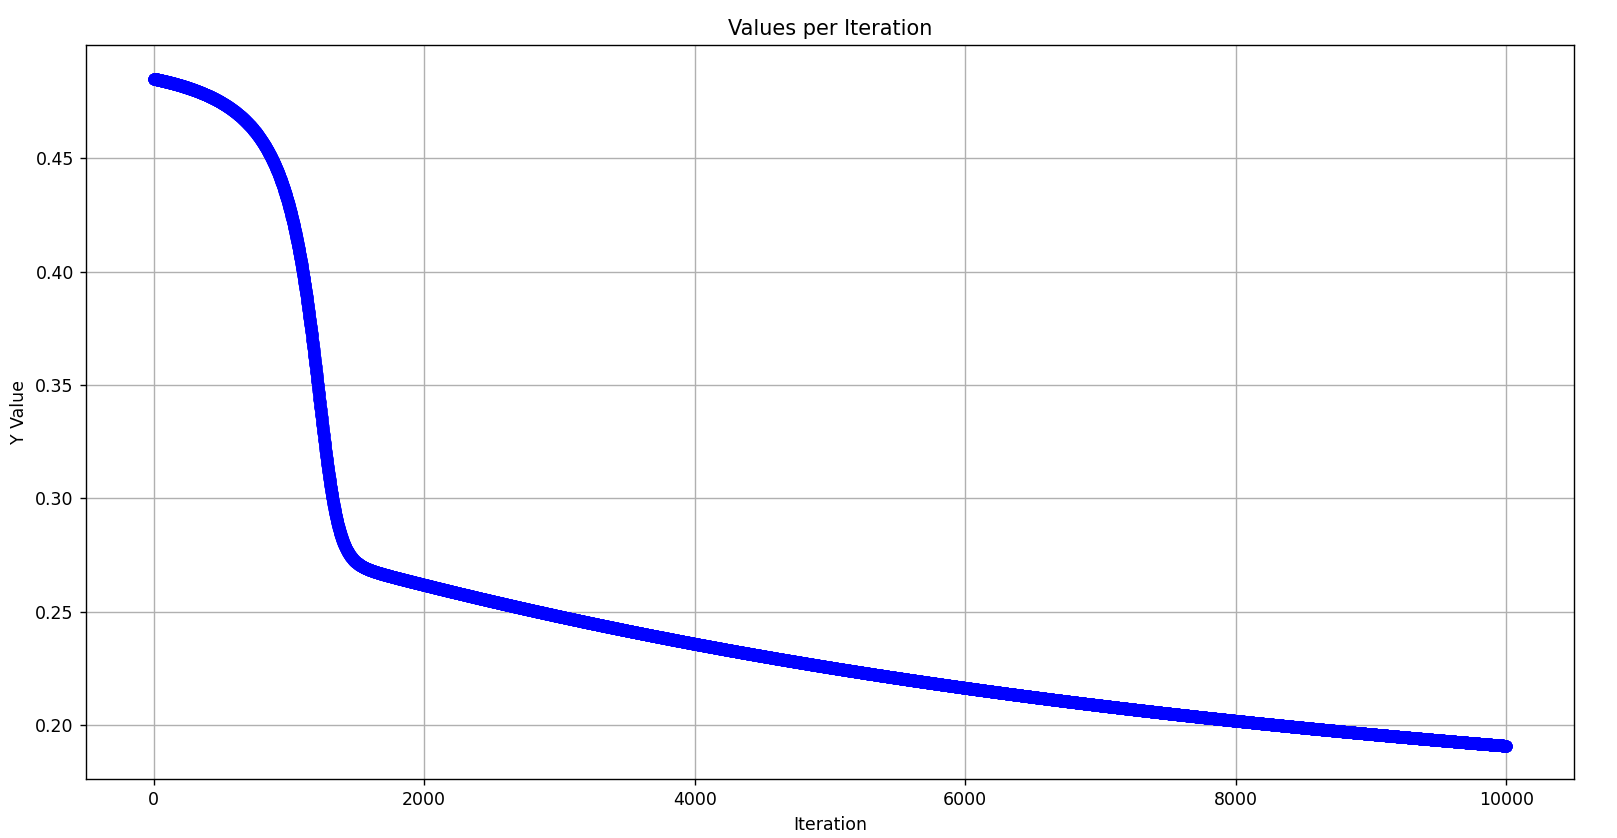
\includegraphics[width=0.7\textwidth]{iris-train-cost.png}
                \caption{Training Cost}
            \end{figure}
            \begin{figure}[H]
                \centering
                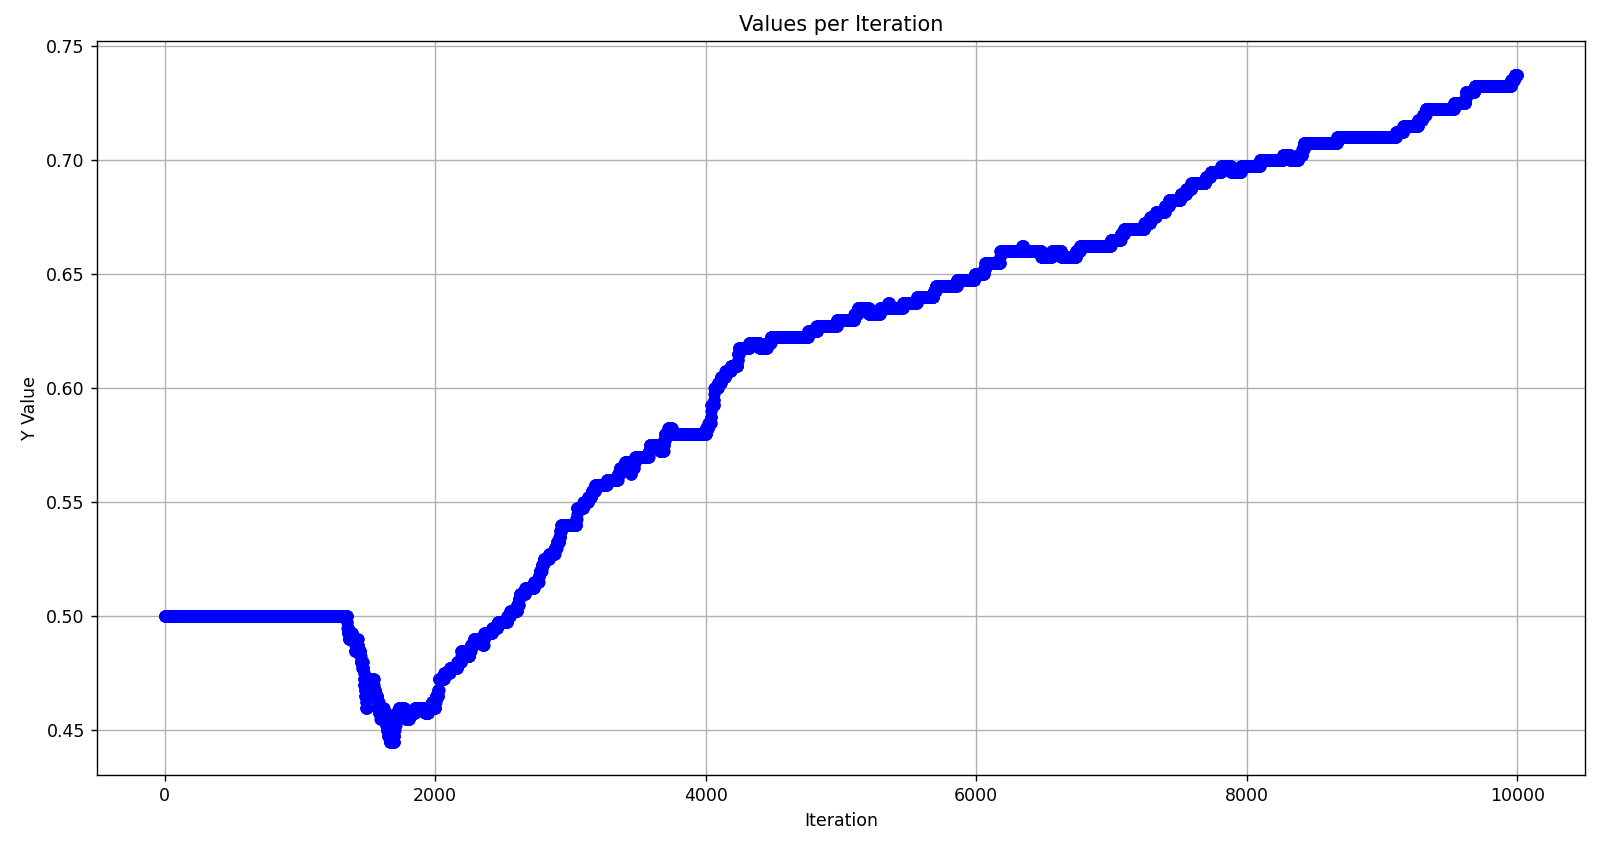
\includegraphics[width=0.7\textwidth]{iris-train-acc.png}
                \caption{Training Accuracy}
            \end{figure}
            \begin{figure}[H]
                \centering
                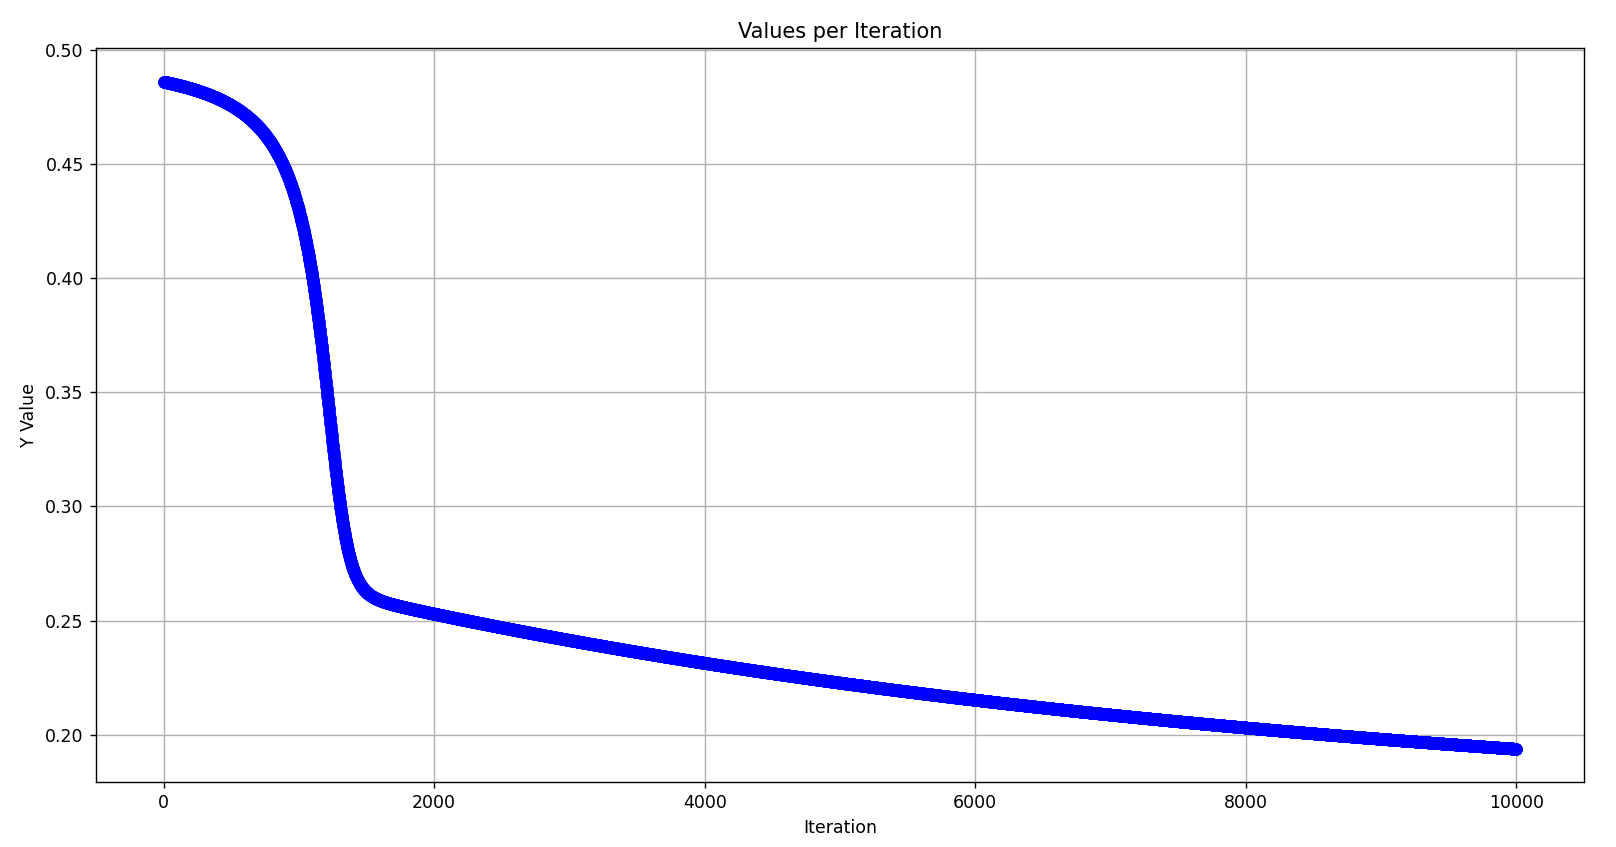
\includegraphics[width=0.7\textwidth]{iris-test-cost.png}
                \caption{Test Cost}
                \label{fig:training-loop}
            \end{figure}
            \begin{figure}[H]
                \centering
                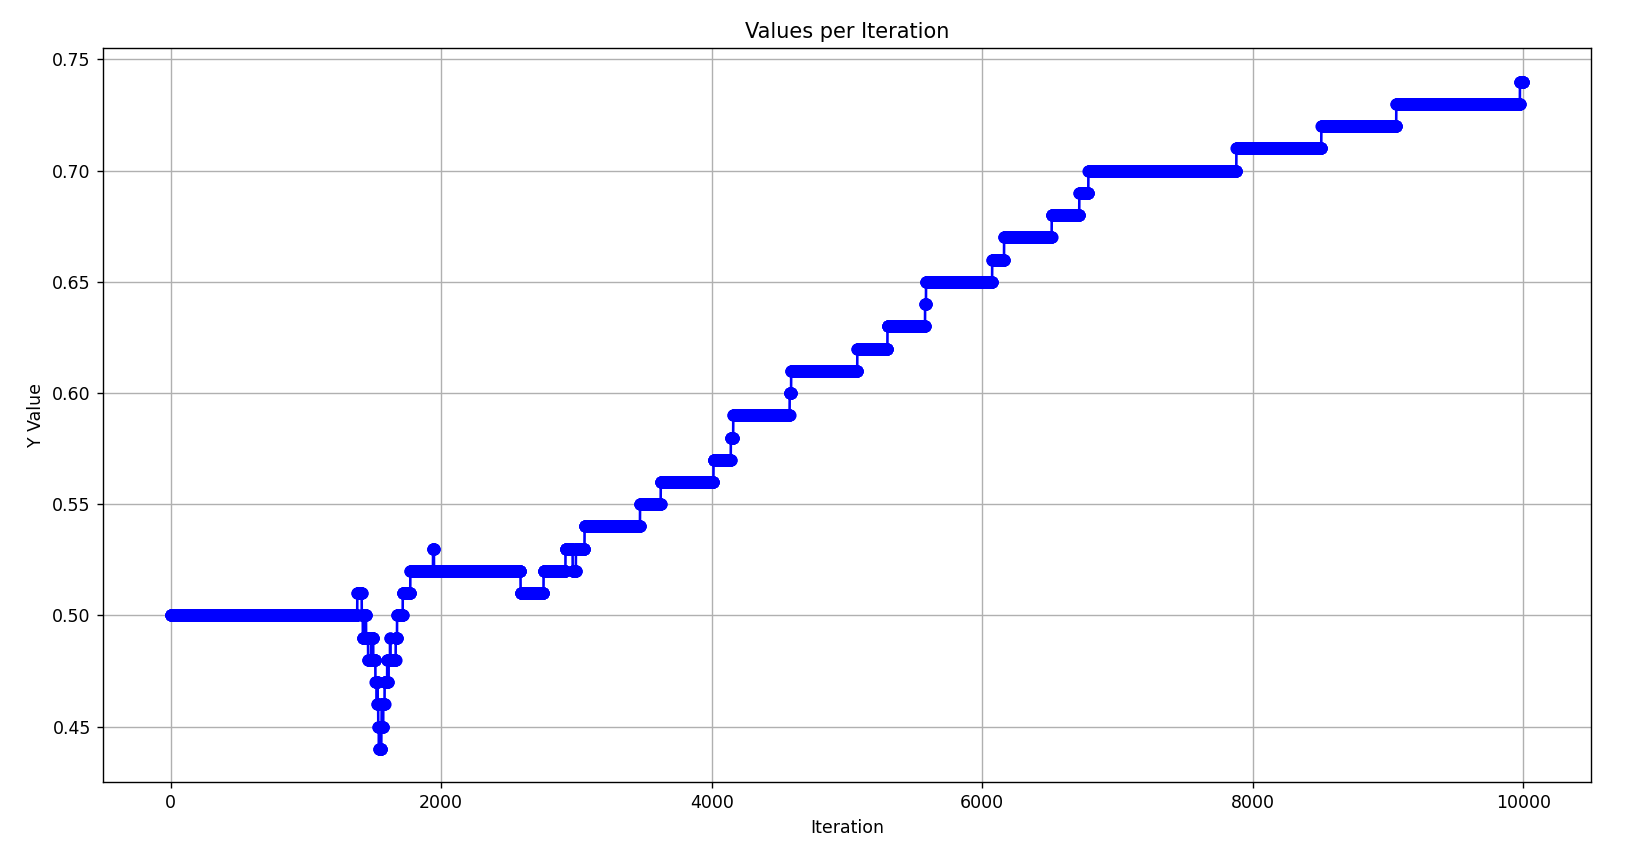
\includegraphics[width=0.7\textwidth]{iris-test-acc.png}
                \caption{Test Accuracy}
            \end{figure}
            The weights and bias obtained using $10000$ epochs and a $0.001$ learning rate can be seen in figure-\ref{fig:iris-results}.
            \begin{figure}[H]
                \centering
                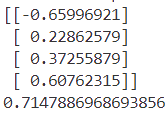
\includegraphics[width=0.4\textwidth]{iris-results.png}
                \caption{$\vec{w}$ and b values}
                \label{fig:iris-results}
            \end{figure}
    \section*{Conclusion}
        After observing the results, we can state that a linear (single neuron) model with a sigmoid activation function worked very well for both the Breast Cancer and Iris datasets. Saddle points and local minimum are a big problem for the current simple implementation of batch gradient descent method, which made the final results very dependent on initial values of $\vec{w}$ and $b$.
    
\end{document}